%% ═══════════════════════════════════════════════════════════════════════════
%% PBEOT504: DATABASE MANAGEMENT SYSTEM — MODULE 2 COMPREHENSIVE STUDY NOTES
%% APJ Abdul Kalam Technological University / CET S5 (2024 Scheme)
%% Styled with Anthropic Notes Design System
%% ═══════════════════════════════════════════════════════════════════════════

\documentclass[11pt,a4paper]{article}

%% ─── Packages ────────────────────────────────────────────────────────────────
\usepackage{fontspec}

%% Font configuration with local fonts and synthetic fallbacks
\setmainfont{Anthropic-serif}[
    Path          = ./,
    Extension     = .ttf,
    AutoFakeBold  = 1.5,
    AutoFakeSlant = 0.2
]
\setsansfont{Poppins}[
    AutoFakeBold  = 1.5,
    AutoFakeSlant = 0.2
]
\setmonofont{DejaVu Sans Mono}[Scale=MatchLowercase]

\usepackage[margin=2.0cm, top=2.5cm, bottom=2.5cm, headheight=25pt]{geometry}
\usepackage[table]{xcolor}
\usepackage{tikz}
\usetikzlibrary{shapes.geometric, arrows.meta, positioning, fit, backgrounds,
                decorations.pathreplacing, calc, patterns}
\usepackage{listings}
\usepackage{tcolorbox}
\tcbuselibrary{listings, skins, breakable, raster}
\usepackage{fancyhdr}
\usepackage{titlesec}
\usepackage{titletoc}
\usepackage{enumitem}
\usepackage{booktabs}
\usepackage{tabularx}
\usepackage{array}
\usepackage{microtype}
\usepackage{hyperref}
\usepackage{amssymb}
\usepackage{amsmath}
\usepackage{parskip}
\usepackage{colortbl}
\usepackage[normalem]{ulem}

%% ─── Document Metadata ──────────────────────────────────────────────────────
\newcommand{\docsubject}{PBEOT504: Database Management System (S5)}
\newcommand{\docshortsubject}{PBEOT504 · Mod 2}
\newcommand{\doctitle}{Relational Model, Relational Algebra \& Advanced SQL}
\newcommand{\docauthor}{Sudheesh}

%% ─── Widow / Orphan Protection ──────────────────────────────────────────────
\widowpenalty=10000
\clubpenalty=10000

%% ─── Spacing ────────────────────────────────────────────────────────────────
\setlength{\parskip}{0.45em plus 0.15em minus 0.1em}
\setlength{\parindent}{0pt}

%% ─── Table Geometry ─────────────────────────────────────────────────────────
\setlength{\aboverulesep}{0pt}
\setlength{\belowrulesep}{0pt}
\setlength{\extrarowheight}{0.65ex}
\renewcommand{\arraystretch}{1.4}
\setlength{\arrayrulewidth}{0.4pt}

\newcolumntype{L}[1]{>{\raggedright\arraybackslash}p{#1}}
\newcolumntype{C}[1]{>{\centering\arraybackslash}p{#1}}
\newcolumntype{R}[1]{>{\raggedleft\arraybackslash}p{#1}}

%% ─── Brand Colors (Anthropic Palette) ────────────────────────────────────────
\definecolor{AnthDark}{HTML}{141413}
\definecolor{AnthLight}{HTML}{faf9f5}
\definecolor{AnthMidGray}{HTML}{7a7870}
\definecolor{AnthLightGray}{HTML}{e8e6dc}
\definecolor{AnthOrange}{HTML}{d97757}
\definecolor{AnthBlue}{HTML}{3b75a4}
\definecolor{AnthGreen}{HTML}{5d7343}
\definecolor{AnthCodeBG}{HTML}{edebe1}
\definecolor{AnthCardBG}{HTML}{f6f5ee}

\arrayrulecolor{AnthMidGray!40}

%% ─── Listings Configuration for SQL ──────────────────────────────────────────
\lstset{
  language        = SQL,
  backgroundcolor = \color{AnthCodeBG},
  basicstyle      = \small\ttfamily\color{AnthDark},
  keywordstyle    = \bfseries\color{AnthBlue},
  stringstyle     = \color{AnthGreen},
  commentstyle    = \itshape\color{AnthMidGray},
  numbers         = none,
  frame           = single,
  rulecolor       = \color{AnthLightGray},
  frameround      = tttt,
  framesep        = 5pt,
  xleftmargin     = 8pt,
  xrightmargin    = 8pt,
  breaklines      = true,
  breakatwhitespace = true,
  showstringspaces= false,
  tabsize         = 2
}

%% ─── Hyperref ────────────────────────────────────────────────────────────────
\hypersetup{
  colorlinks  = true,
  linkcolor   = AnthBlue,
  urlcolor    = AnthOrange,
  citecolor   = AnthGreen,
  pdftitle    = {\doctitle{} · \docsubject},
  pdfauthor   = {\docauthor},
}

%% ─── Page Style ─────────────────────────────────────────────────────────────
\pagestyle{fancy}
\fancyhf{}
\fancyhead[L]{\small\sffamily\color{AnthMidGray}\textbf{\doctitle} \textbar\ \docshortsubject}
\fancyhead[R]{\small\sffamily\color{AnthMidGray}\thepage}
\renewcommand{\headrulewidth}{0.4pt}
\renewcommand{\headrule}{%
  \hbox to\headwidth{\color{AnthOrange}\leaders\hrule height \headrulewidth\hfill}}
\renewcommand{\footrulewidth}{0.4pt}
\renewcommand{\footrule}{%
  \hbox to\headwidth{\color{AnthLightGray}\leaders\hrule height \footrulewidth\hfill}}
\fancyfoot[L]{\footnotesize\sffamily\color{AnthMidGray} APJ Abdul Kalam Technological University (KTU S5)}
\fancyfoot[R]{\footnotesize\sffamily\color{AnthMidGray} PBEOT504 Study Material}

%% ─── Section Formatting ─────────────────────────────────────────────────────
\titleformat{\section}
  {\Large\bfseries\sffamily\color{AnthDark}}
  {\colorbox{AnthOrange}{\makebox[0.65cm][c]{\color{white}\thesection}}\quad}
  {0em}
  {}
  [\vspace{-0.5ex}\color{AnthLightGray}\hrule\vspace{0.4ex}]

\titleformat{\subsection}
  {\large\bfseries\sffamily\color{AnthDark}}
  {\color{AnthBlue}\thesubsection\enspace}
  {0em}{}

\titleformat{\subsubsection}
  {\normalsize\bfseries\sffamily\color{AnthDark}}
  {\color{AnthGreen}\thesubsubsection\enspace}
  {0em}{}

\titlespacing{\section}     {0pt}{1.5em}{0.6em}
\titlespacing{\subsection}  {0pt}{1.1em}{0.3em}
\titlespacing{\subsubsection}{0pt}{0.8em}{0.25em}

%% ─── Table of Contents Styling ──────────────────────────────────────────────
\contentsmargin{0pt}

\titlecontents{section}
  [0pt]
  {\vspace{4pt}\bfseries\sffamily\color{AnthDark}}
  {\colorbox{AnthOrange}{\makebox[0.55cm][c]{\color{white}\small\thecontentslabel}}\enspace}
  {}
  {\hfill\color{AnthOrange}\contentspage}

\titlecontents{subsection}
  [1.5em]
  {\small\sffamily\color{AnthBlue}}
  {\thecontentslabel\enspace}
  {}
  {\titlerule*[6pt]{\tiny\color{AnthMidGray}.}\color{AnthBlue}\contentspage}

\titlecontents{subsubsection}
  [3.5em]
  {\footnotesize\sffamily\color{AnthGreen}}
  {\thecontentslabel\enspace}
  {}
  {\titlerule*[6pt]{\tiny\color{AnthMidGray}.}\color{AnthGreen}\contentspage}

%% ─── tcolorbox Styles ───────────────────────────────────────────────────────
\tcbset{
  notebox/.style={
    enhanced, breakable,
    colback     = AnthCardBG,
    colframe    = AnthMidGray,
    arc=4pt, outer arc=4pt,
    sharp corners=west,
    left=9pt, right=9pt, top=7pt, bottom=7pt,
    boxrule     = 0.5pt,
    colupper    = AnthDark,
    fonttitle   = \bfseries\sffamily\small,
    coltitle    = AnthDark,
    colbacktitle= AnthLightGray,
    borderline west={3pt}{0pt}{AnthMidGray},
    drop fuzzy shadow={AnthMidGray!20},
  },
  tipbox/.style={
    enhanced, breakable,
    colback     = AnthGreen!8,
    colframe    = AnthGreen!70,
    arc=4pt, outer arc=4pt,
    sharp corners=west,
    left=9pt, right=9pt, top=7pt, bottom=7pt,
    boxrule     = 0.5pt,
    colupper    = AnthDark,
    fonttitle   = \bfseries\sffamily\small,
    coltitle    = white,
    colbacktitle= AnthGreen,
    borderline west={3pt}{0pt}{AnthGreen},
    drop fuzzy shadow={AnthGreen!20},
  },
  warnbox/.style={
    enhanced, breakable,
    colback     = AnthOrange!7,
    colframe    = AnthOrange!70,
    arc=4pt, outer arc=4pt,
    sharp corners=west,
    left=9pt, right=9pt, top=7pt, bottom=7pt,
    boxrule     = 0.5pt,
    colupper    = AnthDark,
    fonttitle   = \bfseries\sffamily\small,
    coltitle    = white,
    colbacktitle= AnthOrange,
    borderline west={3pt}{0pt}{AnthOrange},
    drop fuzzy shadow={AnthOrange!20},
  },
  defbox/.style={
    enhanced, breakable,
    colback     = AnthLight,
    colframe    = AnthLightGray,
    arc=4pt, outer arc=4pt,
    sharp corners=west,
    left=9pt, right=9pt, top=7pt, bottom=7pt,
    boxrule     = 0.5pt,
    colupper    = AnthDark,
    borderline west={3.5pt}{0pt}{AnthOrange},
    drop fuzzy shadow={AnthMidGray!20},
  },
  derivbox/.style={
    enhanced, breakable,
    colback     = AnthCardBG!60,
    colframe    = AnthBlue!70,
    arc=4pt, outer arc=4pt,
    sharp corners=west,
    left=9pt, right=9pt, top=7pt, bottom=7pt,
    boxrule     = 0.5pt,
    colupper    = AnthDark,
    fonttitle   = \bfseries\sffamily\small,
    coltitle    = white,
    colbacktitle= AnthBlue,
    borderline west={3.5pt}{0pt}{AnthBlue},
    drop fuzzy shadow={AnthBlue!15},
  },
  problembox/.style={
    enhanced, breakable,
    colback     = AnthBlue!6,
    colframe    = AnthBlue!80,
    arc=4pt, outer arc=4pt,
    sharp corners=west,
    left=9pt, right=9pt, top=7pt, bottom=7pt,
    boxrule     = 0.5pt,
    colupper    = AnthDark,
    fonttitle   = \bfseries\sffamily\small,
    coltitle    = white,
    colbacktitle= AnthBlue,
    borderline west={3.5pt}{0pt}{AnthBlue},
    drop fuzzy shadow={AnthBlue!20},
  },
  solbox/.style={
    enhanced, breakable,
    colback     = AnthLight,
    colframe    = AnthGreen!60,
    arc=4pt, outer arc=4pt,
    sharp corners=west,
    left=9pt, right=9pt, top=7pt, bottom=7pt,
    boxrule     = 0.5pt,
    colupper    = AnthDark,
    fonttitle   = \bfseries\sffamily\small,
    coltitle    = white,
    colbacktitle= AnthGreen!85,
    borderline west={3.5pt}{0pt}{AnthGreen},
    drop fuzzy shadow={AnthGreen!15},
  }
}

%% ─── Inline Helpers & Custom Environments ────────────────────────────────────
\newcommand{\ic}[1]{\mbox{\colorbox{AnthCodeBG}{\footnotesize\ttfamily\textcolor{AnthBlue}{#1}}}}

\newcommand{\concept}[1]{%
  \vspace{3pt}\noindent\textcolor{AnthGreen}{\rule{3.5pt}{10pt}}\enspace
  \textbf{\sffamily\color{AnthDark}#1}\par\vspace{2pt}%
}

\newcommand{\syllabusitem}[1]{%
  \begin{tcolorbox}[enhanced, colback=AnthOrange!8, colframe=AnthOrange, boxrule=0.4pt, arc=3pt, left=7pt, right=7pt, top=3pt, bottom=3pt]
    \small\sffamily\textbf{\color{AnthOrange}Syllabus Requirement:} #1
  \end{tcolorbox}
}

\newcommand{\LeftJoin}{\mathbin{]\mkern-4mu\bowtie}}
\newcommand{\RightJoin}{\mathbin{\bowtie\mkern-4mu[}}
\newcommand{\FullOuterJoin}{\mathbin{]\mkern-4mu\bowtie\mkern-4mu[}}

\newenvironment{Note}[1][Note]{\begin{tcolorbox}[notebox, title=#1]}{\end{tcolorbox}}
\newenvironment{Tip}[1][Key Concept / Design Rule]{\begin{tcolorbox}[tipbox, title=#1]}{\end{tcolorbox}}
\newenvironment{Warn}[1][Important Exam Alert]{\begin{tcolorbox}[warnbox, title=#1]}{\end{tcolorbox}}
\newenvironment{Def}[1][]{\begin{tcolorbox}[defbox]\ifx&#1&\else\textbf{\color{AnthOrange}#1:}\enspace\fi}{\end{tcolorbox}}
\newenvironment{Deriv}[1][Mapping Algorithm]{\begin{tcolorbox}[derivbox, title=#1]}{\end{tcolorbox}}
\newenvironment{Problem}[1][Problem Scenario]{\begin{tcolorbox}[problembox, title=#1]}{\end{tcolorbox}}
\newenvironment{Solution}[1][Step-by-Step Solution]{\begin{tcolorbox}[solbox, title=#1]}{\end{tcolorbox}}

%% ─── Lists Styling ──────────────────────────────────────────────────────────
\setlist[itemize,1]{itemsep=1.5pt, topsep=2pt, parsep=0pt, label={\color{AnthOrange}\small$\blacktriangleright$}}
\setlist[itemize,2]{itemsep=1.5pt, topsep=2pt, parsep=0pt, label={\color{AnthBlue}\small$\blacktriangleright$}}
\setlist[itemize,3]{itemsep=1.5pt, topsep=2pt, parsep=0pt, label={\color{AnthGreen}\small$\blacktriangleright$}}

\setlist[enumerate,1]{itemsep=1.5pt, topsep=2pt, parsep=0pt, label={\bfseries\color{AnthOrange}\arabic*.}}
\setlist[enumerate,2]{itemsep=1.5pt, topsep=2pt, parsep=0pt, label={\bfseries\color{AnthBlue}(\alph*)}}
\setlist[enumerate,3]{itemsep=1.5pt, topsep=2pt, parsep=0pt, label={\color{AnthGreen}\roman*.}}

%% ─── Title Page Macro ───────────────────────────────────────────────────────
\newcommand{\maketitlepage}{%
  \begin{titlepage}
    \pagecolor{AnthDark}
    \color{AnthLight}
    \vspace*{2.2cm}
    \begin{center}
      {\huge\bfseries\sffamily \doctitle}\\[0.8em]
      {\Large\sffamily\color{AnthOrange} \docsubject}\\[0.4em]
      {\large\sffamily\color{AnthMidGray} Bachelor of Technology (B.Tech) — 2024 Scheme}\\[2.0em]
      \color{AnthOrange}\rule{0.5\textwidth}{1.2pt}\\[1.8em]
      {\normalsize\sffamily\color{AnthLightGray} Complete Technical Notes, ER-to-Relational Synthesis \& SQL Query Suite}\\[0.4em]
      {\small\sffamily\color{AnthMidGray} Prepared from Course Materials, Lecture Slides \& KTU Curriculum}\\[2.8em]
      \begin{tcolorbox}[enhanced, width=0.84\textwidth, colback=AnthDark!90, colframe=AnthOrange!60, arc=4pt, boxrule=0.6pt]
        \centering\small\sffamily\color{AnthLight}
        \textbf{Module 2 Complete Syllabus Coverage:}\\[3pt]
        $\bullet$ Structure of Relational Databases: Keys, Integrity Constraints \& Domains\\
        $\bullet$ 7-Step Algorithm for Synthesizing ER Diagrams to Relational Schema\\
        $\bullet$ Relational Algebra: Selection, Projection, Joins, Division \& Complex Queries\\
        $\bullet$ Structured Query Language (SQL): DDL, DML, Nested Queries, Aggregations\\
        $\bullet$ Advanced SQL: Views, Triggers, Assertions, CTEs \& JDBC Host Connectivity\\
        $\bullet$ Comprehensive Problem Suite \& KTU Model Examination Questions
      \end{tcolorbox}
      \vfill
      {\small\sffamily\color{AnthMidGray} Compiled \today}
    \end{center}
    \vspace*{0.8cm}
  \end{titlepage}
  \pagecolor{AnthLight}
  \color{AnthDark}
}

%% ═══════════════════════════════════════════════════════════════════════════
%% DOCUMENT BODY
%% ═══════════════════════════════════════════════════════════════════════════
\begin{document}

\maketitlepage

%% ─── Table of Contents ───────────────────────────────────────────────────────
\thispagestyle{empty}
{
  \hypersetup{hidelinks}
  \tableofcontents
}
\clearpage

%% ─────────────────────────────────────────────────────────────────────────────
\section{Structure of Relational Databases and Integrity Constraints}
%% ─────────────────────────────────────────────────────────────────────────────

\syllabusitem{Structure of Relational Databases - Integrity Constraints, Synthesizing ER diagram to relational schema}

\subsection{Fundamental Concepts of the Relational Model}

Introduced by Dr.~Edgar F.~Codd in 1970 at IBM, the \textbf{Relational Model} represents a database as a collection of mathematically formal two-dimensional tables called \textbf{Relations}.

\begin{center}
\small
\begin{tabularx}{\textwidth}{L{3.5cm} L{3.5cm} X}
  \rowcolor{AnthDark}
  \color{white}\textbf{Formal Relational Term} & \color{white}\textbf{Informal / Practical Term} & \color{white}\textbf{Precise Mathematical Definition} \\
  \rowcolor{AnthCardBG} \textbf{Relation} & Table / File & A subset of the Cartesian product of attribute domains: $R \subseteq \text{dom}(A_1) \times \dots \times \text{dom}(A_n)$ \\
  \textbf{Tuple} & Row / Record & An ordered list of $n$ values $\langle v_1, v_2, \dots, v_n \rangle$ where $v_i \in \text{dom}(A_i)$ \\
  \rowcolor{AnthCardBG} \textbf{Attribute} & Column Header / Field & A named role defining the interpretation of values from domain $\text{dom}(A)$ \\
  \textbf{Domain} & Data Type / Range & Set of atomic, indivisible values permissible for an attribute \\
  \rowcolor{AnthCardBG} \textbf{Degree ($n$)} & Arity / Column Count & The total number of attributes in the relation schema $R(A_1, \dots, A_n)$ \\
  \textbf{Cardinality ($m$)} & Row Count / Record Count & The total number of tuples currently present in relation state $r(R)$ \\
  \rowcolor{AnthCardBG} \textbf{Relation Schema} & Table Structure & Denoted by $R(A_1, A_2, \dots, A_n)$; static description (intension) \\
  \textbf{Relation State} & Table Data / Instance & The set of tuples $r(R) = \{t_1, t_2, \dots, t_m\}$ at a given time (extension) \\
\end{tabularx}
\end{center}

\concept{Characteristics of Relational Databases}
\begin{enumerate}
  \item \textbf{No Duplicate Tuples:} By mathematical definition, a relation is a set of distinct tuples. Duplicate rows are strictly disallowed.
  \item \textbf{Ordering of Tuples is Irrelevant:} Tuples have no inherent physical sequence inside a relation.
  \item \textbf{Ordering of Attributes is Irrelevant:} Attributes are identified by unique column names, not position.
  \item \textbf{Atomicity of Values (First Normal Form - 1NF):} Every attribute value in a tuple must be an indivisible atomic value. Multivalued or composite attributes are forbidden in normalized relational tables.
  \item \textbf{The NULL Value Concept:} Used to represent values that are unknown, missing, or inapplicable.
\end{enumerate}

%% ─────────────────────────────────────────────────────────────────────────────
\subsection{Relational Keys: Taxonomy and Definitions}

Keys are fundamental mathematical constructs that ensure tuple uniqueness and establish relationships between tables.

\begin{Def}[Key Definitions]
\textbf{1. Super Key ($SK$):}
A set of one or more attributes that collectively uniquely identifies a tuple within a relation. For any two distinct tuples $t_1, t_2 \in r(R)$, $t_1[SK] \neq t_2[SK]$. A super key may contain extraneous attributes.

\textbf{2. Candidate Key ($CK$):}
A \textbf{minimal Super Key}. A super key $K$ is a candidate key if removing any attribute from $K$ causes it to lose the uniqueness property. A relation may possess multiple candidate keys.

\textbf{3. Primary Key ($PK$):}
The specific candidate key chosen by the database designer to identify tuples uniquely throughout the database. Its values \textbf{can never be NULL}.

\textbf{4. Alternate Key ($AK$):}
Any candidate key that was \textbf{not chosen} as the primary key ($AK = CK \setminus \{PK\}$).

\textbf{5. Foreign Key ($FK$):}
A set of attributes in a referencing relation $R_1$ whose values are required to match the primary key $PK$ of a referenced relation $R_2$, or else be NULL.
\end{Def}

\begin{center}
\resizebox{0.75\textwidth}{!}{%
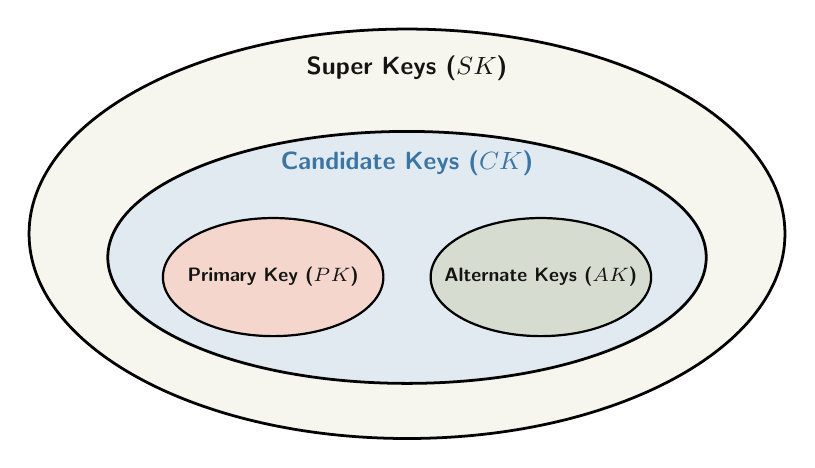
\begin{tikzpicture}
  \draw[line width=1.0pt, fill=AnthCardBG] (0,0) ellipse (4.8cm and 2.6cm);
  \node[font=\small\sffamily\bfseries, color=AnthDark] at (0, 2.1) {Super Keys ($SK$)};

  \draw[line width=1.0pt, fill=AnthBlue!15] (0,-0.3) ellipse (3.8cm and 1.6cm);
  \node[font=\small\sffamily\bfseries, color=AnthBlue] at (0, 0.9) {Candidate Keys ($CK$)};

  \draw[line width=0.8pt, fill=AnthOrange!30] (-1.7,-0.55) ellipse (1.4cm and 0.75cm);
  \node[font=\scriptsize\sffamily\bfseries, color=AnthDark] at (-1.7, -0.55) {Primary Key ($PK$)};

  \draw[line width=0.8pt, fill=AnthGreen!25] (1.7,-0.55) ellipse (1.4cm and 0.75cm);
  \node[font=\scriptsize\sffamily\bfseries, color=AnthDark] at (1.7, -0.55) {Alternate Keys ($AK$)};
\end{tikzpicture}%
}
\end{center}

%% ─────────────────────────────────────────────────────────────────────────────
\subsection{Relational Integrity Constraints}

Integrity constraints are conditions that must hold true on all valid database states.

\begin{enumerate}
  \item \textbf{Domain Constraints:} Every value $t[A]$ must be an atomic value belonging to the domain $\text{dom}(A)$ (data type, length, range restrictions, \ic{CHECK} constraints).
  \item \textbf{Entity Integrity Constraint:} The primary key attributes of a relation schema $R$ \textbf{cannot accept NULL values} ($t[PK] \neq \text{NULL}$ for any tuple $t$). Rationale: NULL values cannot uniquely identify individual tuples.
  \item \textbf{Key / Uniqueness Constraint:} No two tuples in a relation can have identical values for any candidate key ($t_1[CK] \neq t_2[CK]$).
  \item \textbf{Referential Integrity Constraint:} A foreign key $FK$ in relation $R_1$ referencing relation $R_2(PK)$ must satisfy:
    \begin{equation}
      t_1[FK] = t_2[PK] \quad \text{for some } t_2 \in R_2, \quad \text{or} \quad t_1[FK] = \text{NULL}
    \end{equation}
\end{enumerate}

\concept{Handling Violations of Referential Integrity}
When an \ic{UPDATE} or \ic{DELETE} occurs on a referenced table, the DBMS can enforce:
\begin{itemize}
  \item \textbf{\ic{ON DELETE RESTRICT} (or \ic{NO ACTION}):} Rejects the delete operation if child records exist.
  \item \textbf{\ic{ON DELETE CASCADE}:} Automatically deletes all dependent child tuples.
  \item \textbf{\ic{ON DELETE SET NULL}:} Automatically sets the foreign key of child tuples to NULL.
  \item \textbf{\ic{ON DELETE SET DEFAULT}:} Sets the child foreign key to a specified default value.
\end{itemize}

%% ─────────────────────────────────────────────────────────────────────────────
\clearpage
\section{Synthesizing ER Diagrams to Relational Schema}
%% ─────────────────────────────────────────────────────────────────────────────

The logical database design process converts a conceptual ER diagram into a normalized set of relational tables through a rigorous \textbf{7-Step Mapping Algorithm}.

\begin{Deriv}[The 7-Step ER-to-Relational Synthesis Algorithm]
\concept{Step 1: Mapping Strong (Regular) Entity Types}
For each strong entity type $E$, create a relation $R$ containing all simple attributes of $E$.
\begin{itemize}
  \item \textbf{Composite Attributes:} Include only their simple component sub-attributes (e.g., \ic{Name} $\to$ \ic{Fname}, \ic{Minit}, \ic{Lname}).
  \item \textbf{Primary Key:} Primary key of $R =$ primary key of entity $E$.
\end{itemize}

\concept{Step 2: Mapping Weak Entity Types}
For each weak entity type $W$ with identifying owner entity $E$:
\begin{itemize}
  \item Create a relation $R_W$ containing all simple attributes of $W$.
  \item Add the \textbf{Primary Key of $E$} as a \textbf{Foreign Key} in $R_W$.
  \item \textbf{Primary Key of $R_W$:} The composite key $\{ \text{Primary Key of } E \} \cup \{ \text{Partial Key of } W \}$.
\end{itemize}

\concept{Step 3: Mapping Multivalued Attributes}
For each multivalued attribute $A$ in entity $E$:
\begin{itemize}
  \item Create a separate relation $R_A$.
  \item Include attribute $A$ and the \textbf{Primary Key of $E$} (as a Foreign Key).
  \item \textbf{Primary Key of $R_A$:} $\{ \text{Primary Key of } E, A \}$.
\end{itemize}

\concept{Step 4: Mapping Binary 1:1 Relationships}
For a binary $1:1$ relationship between entities $S$ and $T$, choose one of three approaches:
\begin{enumerate}
  \item \textbf{Foreign Key Approach (Standard / Preferred):} Add the primary key of $S$ as a foreign key in $T$ (prefer putting $FK$ in the entity with \textbf{total participation} to prevent NULLs). Include any relationship attributes in $T$.
  \item \textbf{Merged Relation Approach:} If \textbf{both} entities participate totally, merge $S$ and $T$ into a single consolidated relation.
  \item \textbf{Cross-Reference / Junction Relation:} Create a third relation $R(PK_S, PK_T)$ (used if both sides have partial participation).
\end{enumerate}

\concept{Step 5: Mapping Binary 1:N (and N:1) Relationships}
For a $1:N$ relationship between entity $S$ ($1$-side) and entity $T$ ($N$-side):
\begin{itemize}
  \item Identify the relation on the \textbf{$N$-side} ($T$).
  \item Add the \textbf{Primary Key of the $1$-side ($S$)} as a \textbf{Foreign Key} inside relation $T$.
  \item Include any relationship attributes inside $T$.
\end{itemize}

\concept{Step 6: Mapping Binary M:N Relationships}
For an $M:N$ relationship between entities $S$ and $T$:
\begin{itemize}
  \item Create a separate \textbf{Junction / Cross-Reference Relation} $R_{ST}$.
  \item Include the primary key of $S$ ($FK_S$) and primary key of $T$ ($FK_T$) as foreign keys.
  \item \textbf{Primary Key of $R_{ST}$:} The composite key $\{ FK_S, FK_T \}$.
  \item Include all relationship attributes inside $R_{ST}$.
\end{itemize}

\concept{Step 7: Mapping Recursive and N-ary (Ternary) Relationships}
\begin{itemize}
  \item \textbf{Recursive $1:N$ Relationship:} Add a foreign key in the same relation referencing its own primary key (e.g., \ic{EMPLOYEE(SSN, Name, Supervisor\_SSN)}).
  \item \textbf{Ternary / $N$-ary Relationship:} Create a separate relation $R$ containing the foreign keys of all $N$ participating entities plus any relationship attributes. Primary key is the composite of all participating primary keys.
\end{itemize}
\end{Deriv}

%% ─────────────────────────────────────────────────────────────────────────────
\clearpage
\section{Relational Algebra: The Formal Query Language}
%% ─────────────────────────────────────────────────────────────────────────────

\syllabusitem{Relational Algebra - Select, Project, Rename, Set operations, Cartesian Product, Join operations (Inner, Theta, Equi, Natural, Outer Joins), Division operator, Relational Algebra queries}

\subsection{Unary Relational Operators}

Relational algebra is a procedural query language consisting of operations that take one or two relations as input and produce a new relation as output.

\concept{1. The Select Operation ($\sigma$)}
The \textbf{Select} operator ($\sigma$) filters rows (tuples) that satisfy a boolean selection condition:
\begin{equation}
  \sigma_{\langle \text{condition} \rangle}(R) = \{ t \mid t \in R \text{ and } \text{condition}(t) = \text{TRUE} \}
\end{equation}
\begin{itemize}
  \item \emph{Degree:} Same as degree of $R$ ($\text{deg}(\sigma(R)) = \text{deg}(R)$).
  \item \emph{Cardinality:} $|\sigma(R)| \le |R|$.
  \item \emph{Example:} $\sigma_{\text{Age} > 20 \land \text{Branch} = '\text{EEE}'}(\text{STUDENT})$.
\end{itemize}

\concept{2. The Project Operation ($\Pi$)}
The \textbf{Project} operator ($\Pi$) selects specified columns (attributes) and discards the rest:
\begin{equation}
  \Pi_{A_1, A_2, \dots, A_k}(R)
\end{equation}
\begin{itemize}
  \item \emph{Duplicate Elimination:} By definition of a mathematical set, $\Pi$ \textbf{automatically eliminates duplicate tuples} from the resulting relation.
  \item \emph{Example:} $\Pi_{\text{RollNo, Name}}(\sigma_{\text{Age} > 20}(\text{STUDENT}))$.
\end{itemize}

\concept{3. The Rename Operation ($\rho$)}
Used to rename relations or attributes:
\begin{equation}
  \rho_{S(B_1, B_2, \dots, B_n)}(R) \quad \text{or} \quad \rho_S(R)
\end{equation}

%% ─────────────────────────────────────────────────────────────────────────────
\subsection{Set-Theoretic Relational Operators}

Two relations $R(A_1, \dots, A_n)$ and $S(B_1, \dots, B_n)$ are \textbf{Union-Compatible} (type-compatible) if:
\begin{enumerate}
  \item They have the same degree ($\text{deg}(R) = \text{deg}(S) = n$).
  \item The domains of corresponding attributes are identical: $\text{dom}(A_i) = \text{dom}(B_i)$ for all $1 \le i \le n$.
\end{enumerate}

\begin{Def}[Set Operations]
\begin{itemize}
  \item \textbf{Union ($R \cup S$):} Set of all tuples that appear in $R$, in $S$, or in both.
  \item \textbf{Intersection ($R \cap S$):} Set of tuples appearing in both $R$ and $S$ ($R \cap S = R - (R - S)$).
  \item \textbf{Set Difference ($R - S$):} Set of tuples in $R$ that do not appear in $S$.
  \item \textbf{Cartesian Product ($R \times S$):} Combines every tuple in $R$ with every tuple in $S$.
    \begin{equation}
      \text{deg}(R \times S) = \text{deg}(R) + \text{deg}(S), \qquad |R \times S| = |R| \times |S|
    \end{equation}
\end{itemize}
\end{Def}

%% ─────────────────────────────────────────────────────────────────────────────
\subsection{Binary Relational Join Operations}

\concept{1. Theta Join ($\bowtie_\theta$)}
Combines related tuples from two relations satisfying a condition $\theta \in \{ =, <, \le, >, \ge, \neq \}$:
\begin{equation}
  R \bowtie_{\theta} S = \sigma_{\theta}(R \times S)
\end{equation}

\concept{2. Equi-Join}
A theta join where the comparison operator is strictly equality ($=$). Duplicate attribute columns remain in the output schema.

\concept{3. Natural Join ($R \ast S$ or $R \bowtie S$)}
An Equi-Join performed over all common attribute names in $R$ and $S$, followed by \textbf{automatic projection to remove duplicate attribute columns}:
\begin{equation}
  R \bowtie S = \Pi_{\text{Attributes}}( \sigma_{R.A_1 = S.A_1 \land \dots \land R.A_k = S.A_k}(R \times S) )
\end{equation}

\concept{4. Outer Joins (Preserving Dangling Tuples)}
\begin{itemize}
  \item \textbf{Left Outer Join ($R \LeftJoin S$):} Keeps all tuples from left relation $R$. If no match exists in $S$, the $S$-attributes are filled with \ic{NULL}.
  \item \textbf{Right Outer Join ($R \RightJoin S$):} Keeps all tuples from right relation $S$, padding unmatched $R$-attributes with \ic{NULL}.
  \item \textbf{Full Outer Join ($R \FullOuterJoin S$):} Keeps all tuples from both relations, padding unmatched fields with \ic{NULL}.
\end{itemize}

\concept{5. Division Operator ($\div$)}
The \textbf{Division Operator ($R \div S$)} answers queries involving universal quantification ("Find entities associated with \textbf{ALL} items in $S$").
\begin{equation}
  R \div S = \Pi_{A - B}(R) - \Pi_{A - B}\left( (\Pi_{A - B}(R) \times S) - R \right)
\end{equation}
\emph{Condition:} Attributes of $S$ must be a proper subset of attributes of $R$ ($B \subset A$). The result contains attributes $(A - B)$.

%% ─────────────────────────────────────────────────────────────────────────────
\clearpage
\section{Structured Query Language (SQL)}
%% ─────────────────────────────────────────────────────────────────────────────

\syllabusitem{Structured Query Language (SQL), Data Definition Language (DDL), Table definitions and operations – CREATE, DROP, ALTER, INSERT, DELETE, UPDATE. SQL DML - SQL queries on single and multiple tables, Nested queries, Aggregation and grouping, Views, assertions, Triggers, SQL data types, Recursive queries, Accessing SQL from a Programming Language}

\subsection{SQL Data Definition Language (DDL)}

\concept{1. Table Creation with Comprehensive Constraints}
\begin{lstlisting}
CREATE TABLE DEPARTMENT (
    DNumber     INT PRIMARY KEY,
    DName       VARCHAR(50) NOT NULL UNIQUE,
    Manager_SSN CHAR(9),
    Mgr_Start_Date DATE
);

CREATE TABLE EMPLOYEE (
    SSN         CHAR(9) PRIMARY KEY,
    FName       VARCHAR(30) NOT NULL,
    LName       VARCHAR(30) NOT NULL,
    Salary      DECIMAL(10,2) CHECK (Salary >= 10000.00),
    DNo         INT NOT NULL,
    Supervisor_SSN CHAR(9),
    FOREIGN KEY (DNo) REFERENCES DEPARTMENT(DNumber) 
        ON DELETE CASCADE ON UPDATE CASCADE,
    FOREIGN KEY (Supervisor_SSN) REFERENCES EMPLOYEE(SSN) 
        ON DELETE SET NULL ON UPDATE CASCADE
);
\end{lstlisting}

\concept{2. Schema Modification and Table Deletion}
\begin{lstlisting}
-- Add new column
ALTER TABLE EMPLOYEE ADD Email VARCHAR(100);

-- Modify column data type
ALTER TABLE EMPLOYEE MODIFY Salary DECIMAL(12,2);

-- Drop table and related constraints
DROP TABLE EMPLOYEE CASCADE;

-- Delete all rows while preserving table structure
TRUNCATE TABLE EMPLOYEE;
\end{lstlisting}

%% ─────────────────────────────────────────────────────────────────────────────
\subsection{SQL Data Manipulation Language (DML)}

\begin{lstlisting}
-- Insert single row
INSERT INTO EMPLOYEE (SSN, FName, LName, Salary, DNo) 
VALUES ('123456789', 'John', 'Smith', 55000.00, 5);

-- Update tuples conditionally
UPDATE EMPLOYEE 
SET Salary = Salary * 1.10 
WHERE DNo = 5;

-- Delete tuples conditionally
DELETE FROM EMPLOYEE 
WHERE Salary < 20000.00;
\end{lstlisting}

%% ─────────────────────────────────────────────────────────────────────────────
\subsection{Advanced SQL Retrieval: Joins, Nested Queries, and Aggregations}

\concept{1. The SELECT-FROM-WHERE Framework and Multi-Table Joins}
\begin{lstlisting}
-- Find Employee Names and their Department Names (Explicit Inner Join)
SELECT E.FName, E.LName, D.DName 
FROM EMPLOYEE E 
JOIN DEPARTMENT D ON E.DNo = D.DNumber 
WHERE E.Salary > 40000.00;
\end{lstlisting}

\concept{2. Aggregate Functions, GROUP BY, and HAVING Clause}
\begin{itemize}
  \item \textbf{Aggregate Functions:} \ic{COUNT()}, \ic{SUM()}, \ic{AVG()}, \ic{MIN()}, \ic{MAX()}.
  \item \textbf{WHERE vs. HAVING:} \ic{WHERE} filters individual rows \emph{before} grouping; \ic{HAVING} filters aggregated groups \emph{after} grouping.
\end{itemize}
\begin{lstlisting}
-- Find Departments having more than 5 employees with average salary > 50000
SELECT DNo, COUNT(*) AS Total_Employees, AVG(Salary) AS Avg_Salary 
FROM EMPLOYEE 
WHERE Salary >= 20000.00 
GROUP BY DNo 
HAVING COUNT(*) > 5 AND AVG(Salary) > 50000.00;
\end{lstlisting}

\concept{3. Nested Subqueries: Non-Correlated vs. Correlated}
\begin{lstlisting}
-- Non-Correlated Subquery using IN
SELECT FName, LName FROM EMPLOYEE 
WHERE DNo IN (SELECT DNumber FROM DEPARTMENT WHERE DName = 'Research');

-- Correlated Subquery using EXISTS (Employees who work on all department projects)
SELECT E.FName, E.LName FROM EMPLOYEE E 
WHERE NOT EXISTS (
    SELECT P.PNumber FROM PROJECT P WHERE P.DNum = E.DNo 
    EXCEPT 
    SELECT W.PNo FROM WORKS_ON W WHERE W.ESSN = E.SSN
);
\end{lstlisting}

%% ─────────────────────────────────────────────────────────────────────────────
\subsection{Views, Assertions, Triggers, and Recursive Queries}

\concept{1. Views: Virtual Tables}
A \textbf{View} is a dynamic virtual table defined by an underlying SQL query. It does not store physical data independently:
\begin{lstlisting}
CREATE VIEW EEE_DEPT_EMPS AS 
SELECT E.SSN, E.FName, E.LName, E.Salary 
FROM EMPLOYEE E 
WHERE E.DNo = (SELECT DNumber FROM DEPARTMENT WHERE DName = 'EEE');
\end{lstlisting}
\emph{Benefits:} Security abstraction, simplified complex queries, logical data independence.

\concept{2. Database Triggers (Event-Condition-Action / ECA Model)}
\begin{lstlisting}
CREATE TRIGGER check_min_salary 
BEFORE INSERT ON EMPLOYEE 
FOR EACH ROW 
BEGIN 
    IF NEW.Salary < 15000.00 THEN 
        SIGNAL SQLSTATE '45000' 
        SET MESSAGE_TEXT = 'Salary cannot be less than minimum wage 15000!';
    END IF; 
END;
\end{lstlisting}

\concept{3. Recursive Queries using Common Table Expressions (CTE)}
\begin{lstlisting}
-- Find the complete management hierarchy under CEO
WITH RECURSIVE OrgHierarchy AS (
    -- Anchor Member
    SELECT SSN, FName, Supervisor_SSN, 1 AS Level 
    FROM EMPLOYEE WHERE Supervisor_SSN IS NULL 
    UNION ALL 
    -- Recursive Member
    SELECT E.SSN, E.FName, E.Supervisor_SSN, O.Level + 1 
    FROM EMPLOYEE E 
    JOIN OrgHierarchy O ON E.Supervisor_SSN = O.SSN
)
SELECT * FROM OrgHierarchy;
\end{lstlisting}

\concept{4. Accessing SQL from Programming Languages: JDBC Architecture}
Java DataBase Connectivity (\textbf{JDBC}) is a standard Java API that enables Java programs to execute SQL statements.
\begin{enumerate}
  \item \textbf{\ic{DriverManager}:} Manages database drivers and establishes database connections.
  \item \textbf{\ic{Connection}:} Represents an active session with the specific database.
  \item \textbf{\ic{PreparedStatement}:} Pre-compiled SQL statements preventing SQL Injection attacks.
  \item \textbf{\ic{ResultSet}:} Cursor-based data structure used to iterate through rows retrieved by a query.
\end{enumerate}

%% ─────────────────────────────────────────────────────────────────────────────
\clearpage
\section{Comprehensive Relational \& SQL Problem Suite}
%% ─────────────────────────────────────────────────────────────────────────────

\begin{Problem}[Problem 1: Synthesizing Complex ER Diagram to Relational Schema]
Convert the following University ER scenario into a normalized Relational Database Schema:
\begin{itemize}
  \item \ic{PROFESSOR}(\underline{EmpNo}, Name, Designation)
  \item \ic{DEPARTMENT}(\underline{Dept\_ID}, Dept\_Name). A department offers multiple courses. A course is offered by exactly 1 department.
  \item \ic{COURSE}(\underline{CourseID}, Course\_Name, Credits). Has multivalued attribute \ic{Prerequisites}.
  \item \ic{STUDENT}(\underline{RollNo}, Name, Address(Street, City, Pincode), Phone\_Numbers).
  \item Relationships: \ic{TEACHES} ($M:N$ between \ic{PROFESSOR} and \ic{COURSE} with attribute \ic{Semester}), \ic{ENROLLS} ($M:N$ between \ic{STUDENT} and \ic{COURSE} with attribute \ic{Grade}).
\end{itemize}
\end{Problem}

\begin{Solution}
Applying the 7-Step Synthesis Algorithm:
\begin{enumerate}
  \item \textbf{\ic{DEPARTMENT}}(\underline{Dept\_ID}, Dept\_Name)
  \item \textbf{\ic{PROFESSOR}}(\underline{EmpNo}, Name, Designation, Dept\_ID$_{\text{FK}}$)
  \item \textbf{\ic{COURSE}}(\underline{CourseID}, Course\_Name, Credits, Dept\_ID$_{\text{FK}}$)
  \item \textbf{\ic{COURSE\_PREREQUISITES}}(\underline{CourseID}$_{\text{FK}}$, \underline{Prereq\_CourseID}$_{\text{FK}}$)
  \item \textbf{\ic{STUDENT}}(\underline{RollNo}, Name, Street, City, Pincode)
  \item \textbf{\ic{STUDENT\_PHONES}}(\underline{RollNo}$_{\text{FK}}$, \underline{Phone\_Number})
  \item \textbf{\ic{TEACHES}}(\underline{EmpNo}$_{\text{FK}}$, \underline{CourseID}$_{\text{FK}}$, \underline{Semester})
  \item \textbf{\ic{ENROLLS}}(\underline{RollNo}$_{\text{FK}}$, \underline{CourseID}$_{\text{FK}}$, Grade)
\end{enumerate}
\end{Solution}

\begin{Problem}[Problem 2: Relational Algebra Query Suite on University Schema]
Given the schema:
\begin{itemize}
  \item $\text{STUDENT}(\underline{\text{RollNo}}, \text{Name}, \text{Age}, \text{Gender})$
  \item $\text{COURSE}(\underline{\text{CourseID}}, \text{CName}, \text{Credits})$
  \item $\text{ENROLLS}(\underline{\text{RollNo}}, \underline{\text{CourseID}}, \text{Grade})$
  \item $\text{PROFESSOR}(\underline{\text{EmpNo}}, \text{PName}, \text{Phone})$
  \item $\text{TEACHES}(\underline{\text{EmpNo}}, \underline{\text{CourseID}})$
\end{itemize}
Write relational algebra expressions for:
\begin{enumerate}
  \item Find the Credits of course with name \ic{'DBMS'}.
  \item Find RollNo, Name, and Gender of students enrolled in \ic{'Chemistry'}.
  \item Find Names and Phone numbers of professors who taught at least one course.
  \item Find RollNo and Names of students who enrolled in \textbf{ALL} courses.
\end{enumerate}
\end{Problem}

\begin{Solution}
\begin{enumerate}
  \item $\Pi_{\text{Credits}}\left( \sigma_{\text{CName} = '\text{DBMS}'}(\text{COURSE}) \right)$
  \item $\Pi_{\text{RollNo, Name, Gender}}\left( \text{STUDENT} \bowtie \text{ENROLLS} \bowtie \sigma_{\text{CName} = '\text{Chemistry}'}(\text{COURSE}) \right)$
  \item $\Pi_{\text{PName, Phone}}\left( \text{PROFESSOR} \bowtie \text{TEACHES} \right)$
  \item $\Pi_{\text{RollNo, Name}}\left( \text{STUDENT} \bowtie \left( \Pi_{\text{RollNo, CourseID}}(\text{ENROLLS}) \div \Pi_{\text{CourseID}}(\text{COURSE}) \right) \right)$
\end{enumerate}
\end{Solution}

\begin{Problem}[Problem 3: Advanced SQL Queries with Aggregations and Subqueries]
Using the University schema, write SQL queries for:
\begin{enumerate}
  \item Find the names of students who have enrolled in courses with more than 3 credits and received grade 'A'.
  \item Find the CourseID and CName of courses that have more than 30 students enrolled.
  \item Find professors who have never taught any course.
  \item For each department, display Dept\_Name and average salary of professors in that department.
\end{enumerate}
\end{Problem}

\begin{Solution}
\begin{lstlisting}
-- Query 1
SELECT S.Name 
FROM STUDENT S 
JOIN ENROLLS E ON S.RollNo = E.RollNo 
JOIN COURSE C ON E.CourseID = C.CourseID 
WHERE C.Credits > 3 AND E.Grade = 'A';

-- Query 2
SELECT C.CourseID, C.CName, COUNT(E.RollNo) AS Student_Count 
FROM COURSE C 
JOIN ENROLLS E ON C.CourseID = E.CourseID 
GROUP BY C.CourseID, C.CName 
HAVING COUNT(E.RollNo) > 30;

-- Query 3
SELECT PName FROM PROFESSOR 
WHERE EmpNo NOT IN (SELECT EmpNo FROM TEACHES);

-- Query 4
SELECT D.Dept_Name, AVG(P.Salary) AS Avg_Salary 
FROM DEPARTMENT D 
JOIN PROFESSOR P ON D.Dept_ID = P.Dept_ID 
GROUP BY D.Dept_ID, D.Dept_Name;
\end{lstlisting}
\end{Solution}

%% ─────────────────────────────────────────────────────────────────────────────
\clearpage
\section{Quick Revision Sheet \& Model Examination Questions}
%% ─────────────────────────────────────────────────────────────────────────────

\subsection{Master Summary Table: Relational Algebra Operators vs. SQL Constructs}

\begin{center}
\small
\begin{tabularx}{\textwidth}{L{2.8cm} L{3.5cm} L{3.5cm} X}
  \rowcolor{AnthDark}
  \color{white}\textbf{Relational Operator} & \color{white}\textbf{Algebraic Notation} & \color{white}\textbf{Equivalent SQL Clause} & \color{white}\textbf{Core Mathematical Behavior} \\
  \rowcolor{AnthCardBG} \textbf{Selection} & $\sigma_{\langle \text{cond} \rangle}(R)$ & \ic{SELECT * WHERE cond} & Horizontal tuple filter \\
  \textbf{Projection} & $\Pi_{\langle \text{attrs} \rangle}(R)$ & \ic{SELECT DISTINCT attrs} & Vertical column extraction \\
  \rowcolor{AnthCardBG} \textbf{Cartesian Product} & $R \times S$ & \ic{CROSS JOIN} & Combines every row in $R$ with $S$ \\
  \textbf{Theta Join} & $R \bowtie_\theta S$ & \ic{JOIN ... ON cond} & Cross product followed by $\sigma_\theta$ \\
  \rowcolor{AnthCardBG} \textbf{Natural Join} & $R \bowtie S$ & \ic{NATURAL JOIN} & Equi-join on common attribute names \\
  \textbf{Left Outer Join} & $R \LeftJoin S$ & \ic{LEFT OUTER JOIN} & Preserves all left tuples; pads with NULL \\
  \rowcolor{AnthCardBG} \textbf{Set Union} & $R \cup S$ & \ic{UNION} & Requires union-compatible schemas \\
  \textbf{Set Difference} & $R - S$ & \ic{EXCEPT} / \ic{MINUS} & Tuples in $R$ not in $S$ \\
  \rowcolor{AnthCardBG} \textbf{Division Operator} & $R \div S$ & \ic{NOT EXISTS ... EXCEPT} & Universal quantification ("for ALL in S") \\
\end{tabularx}
\end{center}

\subsection{Model Examination Questions (KTU S5 Pattern)}

\begin{Warn}[University Examination Pattern (PBEOT504 Scheme)]
The End Semester Examination consists of \textbf{Part A} (8 compulsory questions of 2 marks each, 2 from each module) and \textbf{Part B} (Module choice questions carrying 6 marks each).
\end{Warn}

\concept{Part A: Short Answer Questions (2 Marks Each)}
\begin{enumerate}
  \item \textbf{Q1:} Differentiate between a \emph{Candidate Key} and a \emph{Super Key}. Can a primary key contain a NULL value?
  \item \textbf{Q2:} State the \emph{Entity Integrity Constraint} and \emph{Referential Integrity Constraint} with mathematical formulations.
  \item \textbf{Q3:} Differentiate between \emph{Equi-Join} and \emph{Natural Join} in Relational Algebra.
  \item \textbf{Q4:} What is the purpose of the \emph{Division Operator} ($\div$) in Relational Algebra? Give an example.
  \item \textbf{Q5:} Explain the difference between \ic{WHERE} and \ic{HAVING} clauses in SQL.
  \item \textbf{Q6:} What is a \emph{View} in SQL? State two advantages of using views.
\end{enumerate}

\concept{Part B: Long Answer / Analytical Questions (6 Marks Each)}
\begin{enumerate}
  \item \textbf{Q7 (a):} State and explain the 7-step mapping algorithm to synthesize an ER diagram into a relational schema. \hfill (4 Marks) \\
  \textbf{Q7 (b):} How are weak entities and multivalued attributes mapped into relational tables? \hfill (2 Marks)
  
  \item \textbf{Q8 (a):} Consider the schema: $\text{SAILOR}(\underline{\text{sid}}, \text{sname}, \text{rating}, \text{age})$, $\text{BOAT}(\underline{\text{bid}}, \text{bname}, \text{color})$, and $\text{RESERVES}(\underline{\text{sid}}, \underline{\text{bid}}, \underline{\text{day}})$. Write Relational Algebra queries to: \\
  (i) Find names of sailors who reserved a red boat. \\
  (ii) Find names of sailors who reserved \textbf{all} boats. \hfill (6 Marks)

  \item \textbf{Q9 (a):} Explain the architecture of JDBC. Write the key Java code steps to establish a connection and execute a \ic{PreparedStatement} query. \hfill (6 Marks)
\end{enumerate}

\vfill
\begin{center}
\small\sffamily\color{AnthMidGray}
--- End of Module 2 Study Notes ---
\end{center}

\end{document}
